\chapter{Physics simulation of proton collisions}
\label{chapter:EventSim}

Proton collisions are complex processes and their understanding is essential to interpret the experimental data from the \acrshort{LHClabel}. Normally, physics analyses rely on the ability to accurately simulate the various processes of proton-proton collisions and the interactions with the detector in order to perform comparisons with the recorded data and quantify the level of agreement with the \acrshort{SMlabel}. The simulation is usually performed with \acrlong{MClabel}~(\acrshort{MClabel}) generators, which are stochastic tools that incorporate both theoretical predictions and empirical results to describe the statistical processes.\\

The simulation of proton-proton interactions is summarised in this chapter, with an overview of each of the steps, starting from the theoretical foundations, computational methods, \acrshort{MClabel} generators and finally with the simulation of the~\acrshort{ATLASlabel} detector.

\section{Event simulation}

A typical proton-proton collision at the LHC is depicted in Figure~\ref{figEVNTSIM:MCsim}. The inelastic scattering is the main interesting process, where the energy of the system is large enough and a constituent of each proton (parton) interacts, generating new particles. The interaction that involves any of the other partons, normally at lower energies, is referred to as underlying event.\\

A key phenomenon is the parton shower, a process where, due to the strong interaction, particles lose energy due to the radiation of gluons, which further generate quark-antiquark pairs, which in turn radiate gluons again in a chain reaction. These generated particles lose energy progressively down to the point where \acrshort{QCD} leaves the perturbative regime ($\sim$1~GeV) and the hadronisation occurs, when quarks and gluons form hadrons, colourless bound states.\\

To complete the simulation of the collision, the pile-up is included, which adds the effects from the other proton collisions that originate from the same or previous bunch-crossing.  

\begin{figure}[htbp]
    \RawFloats
    \begin{center}
    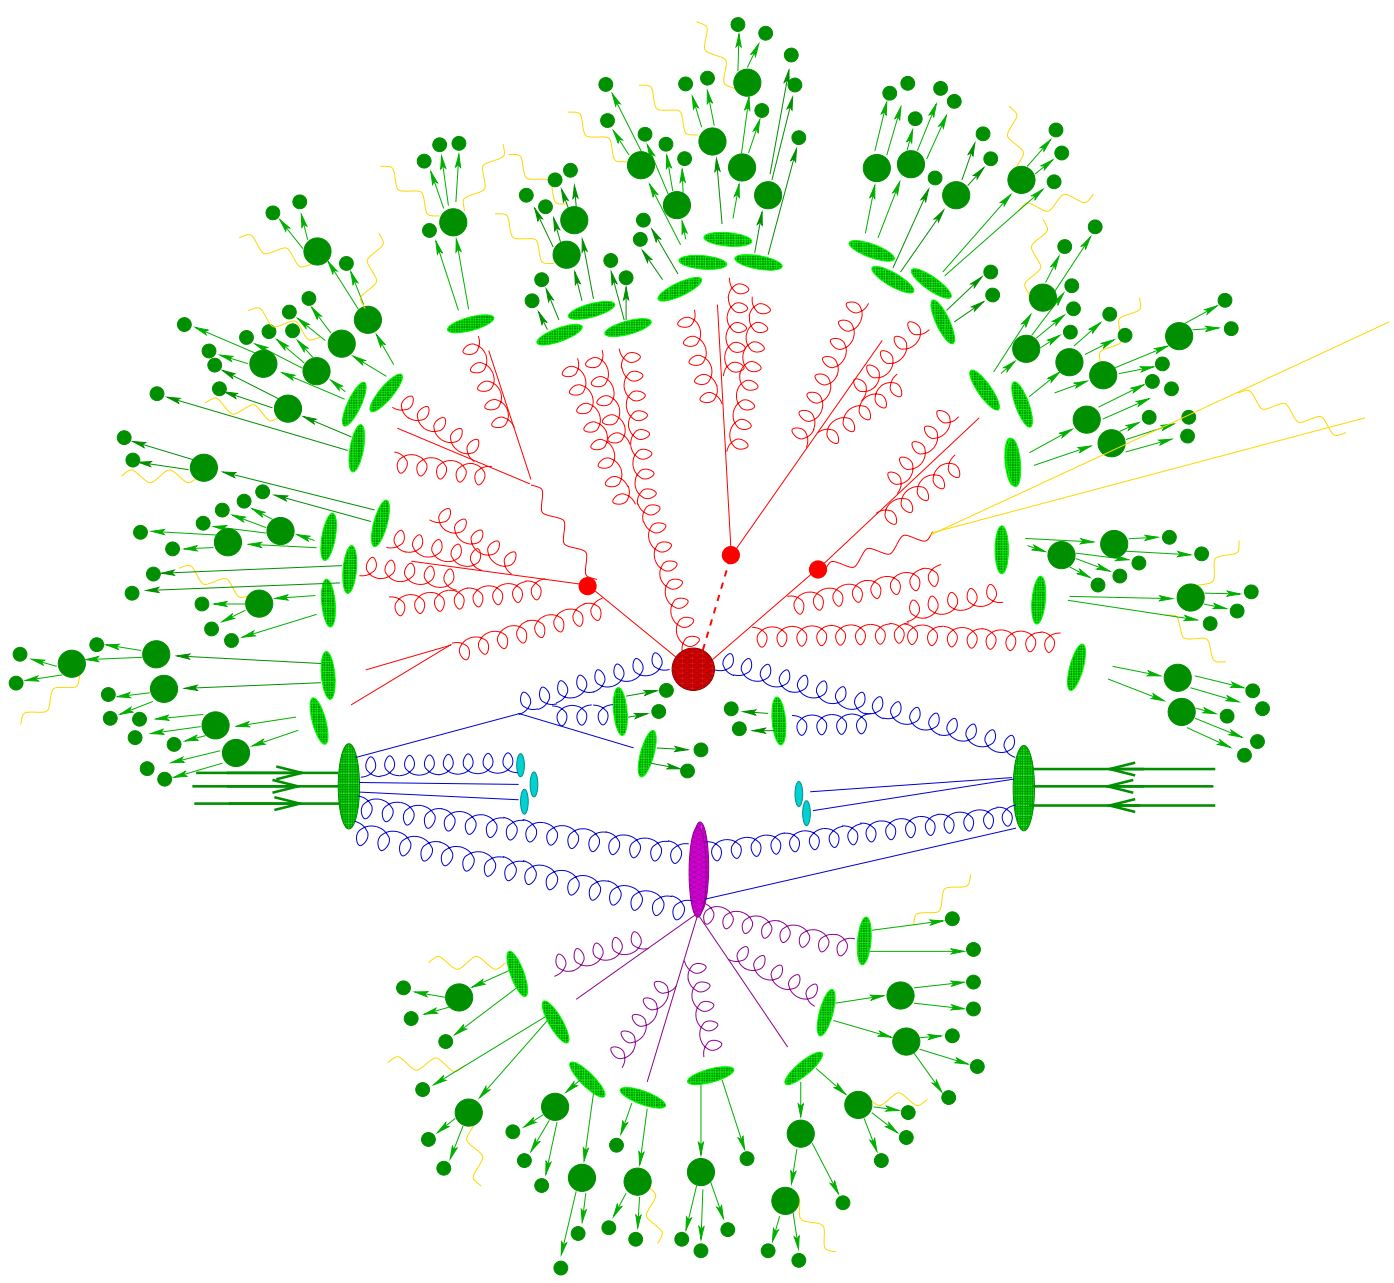
\includegraphics[width=1.0\textwidth]{EVENTSIM/MCsim.JPG}
    \caption{
        Illustration of a proton-proton collision as simulated by a Monte-Carlo event generator. The hard interaction (red blob in the center) is produced from the initial-state partons from the protons (blue), followed by the decay of two top-quarks and a Higgs boson (small red blobs). Additional QCD radiation is produced both before (red) and after (dark green) the final-state partons hadronise. The light green blobs correspond to the hadronisation process of the produced particles and the cyan blobs correspond to the hadronistation of the partons from the proton that did not interact. Also, a secondary interaction (purple) and photon radiation (yellow) are represented. No pile-up effects are illustrated~\cite{Gleisberg_2009}.
    }
    \label{figEVNTSIM:MCsim}
    \end{center}
\end{figure}

\clearpage

\subsection{Factorisation theorem}

The cross-section to produce a final state $X$ from the hard scattering of two protons, $\sigma_{pp\to X}$ can be factorised into two components in perturbation theory, as the strong coupling constant, $\alpha_s$, is small at high energy kinematic regimes. Using the factorisation theorem~\cite{Factorisation},

\begin{equation}
    \sigma_{pp\to X}=\sum_{a,b}\int \text{d}x_a\text{d}x_b f_a(x_a,\mu_F^2)f_b(x_b,\mu_F^2)\cdot\hat{\sigma}_{ab\to X}(x_a p_a,x_b p_b,\mu_F^2,\mu_R^2),
\end{equation}

where $f_i(x_i,\mu_F^2)$ are the \acrlong{PDFlabel}~(\acrshort{PDFlabel}) for partons $i=a,b\in\left\{g, u, \bar{u}, d, ...\right\}$ and encode the probability of finding a parton of type $i$ within the proton carrying a fraction of the proton's momentum $x_i$ at the factorisation scale $\mu_F$. The dependence of the scale appears from performing only fixed-order calculations and the value is typically set comparable to the energy of the process, for example, to the total transverse mass of the final-state particles. The partonic cross-section, $\hat{\sigma}_{ab\to X}(x_a p_a,x_b p_b,\mu_F^2,\mu_R^2)$, is calculated at finite perturbative order, hence the additional dependence on the renormalisation scale, $\mu_R$, at which to evaluate $\alpha_s$.


\subsection{Parton density function}

The \acrshort{PDFlabel}s are crucial for the accurate description of the partons that form the protons. The first type of partons are the valence quarks which determine the quantum numbers of the proton. In addition, gluons and virtual quark-antiquark pairs (sea-quarks) are also part of the proton and come from vacuum fluctuations. A \acrshort{PDFlabel}, $f_i^A(x_i,Q^2)$ describes the probability density of a parton of a certain type, $i$, inside a given hadron, $A$, to carry a certain momentum fraction, $x_i=p_i/p_A$ evaluated at a specific momentum transfer $Q^2$.\\

In general, the \acrshort{PDFlabel}s are extracted from empirical measurements performed at a specific scale. Then, the \acrlong{DGLAPlabel}~(\acrshort{DGLAPlabel}) equations~\cite{DGLAP1,DGLAP2,DGLAP3} are used to extrapolate the \acrshort{PDFlabel} to different scales. Other alternatives to extract the functions like using lattice \acrshort{QCD} are possible, but very computationally challenging~\cite{Bhat_2021}.\\

There are dedicated collaborations such as the \textit{NNPDF}, \textit{CTEQ} and \textit{MSTW} that provide~\cite{Ball_2015,LesHouches,Martin_2009}
 \acrshort{PDFlabel}s for physics analyses. Figure~\ref{figEVNTSIM:PDF} shows the \textit{NNPDF3.0NLO} \acrshort{PDFlabel} set for the different proton partons and two different factorisation scales.\\

 There are two main factorisation schemes that describe processes involving $b$-quarks: the \acrlong{4FSlabel}~(\acrshort{4FSlabel}) and the \acrlong{5FSlabel}~(\acrshort{5FSlabel}). The \acrshort{4FSlabel} treats the $b$-quarks massive ($m_b>\mu_R$) and, since $m_b>m_p$, they are not included in the sea of quarks and do not have an associated \acrshort{PDFlabel}. In the context of \acrshort{QCD} perturbative evolution, one of the consequences is that calculations at lower scales $\mu_R<m_b$ are especially impacted as the $\alpha_s$ running depends on the number of quark flavours in the initial state, $n_f=4$ (Equation~\ref{Theory_eq:runningcoupling}). On the other hand, at high scales the mass effects are negligible and usually described by the \acrshort{5FSlabel}, in which the $b$-quark is considered massless, included in the initial state and treated as the other quarks, $n_f=5$. 

 \begin{figure}[hbtp]
    \RawFloats
    \begin{center}
    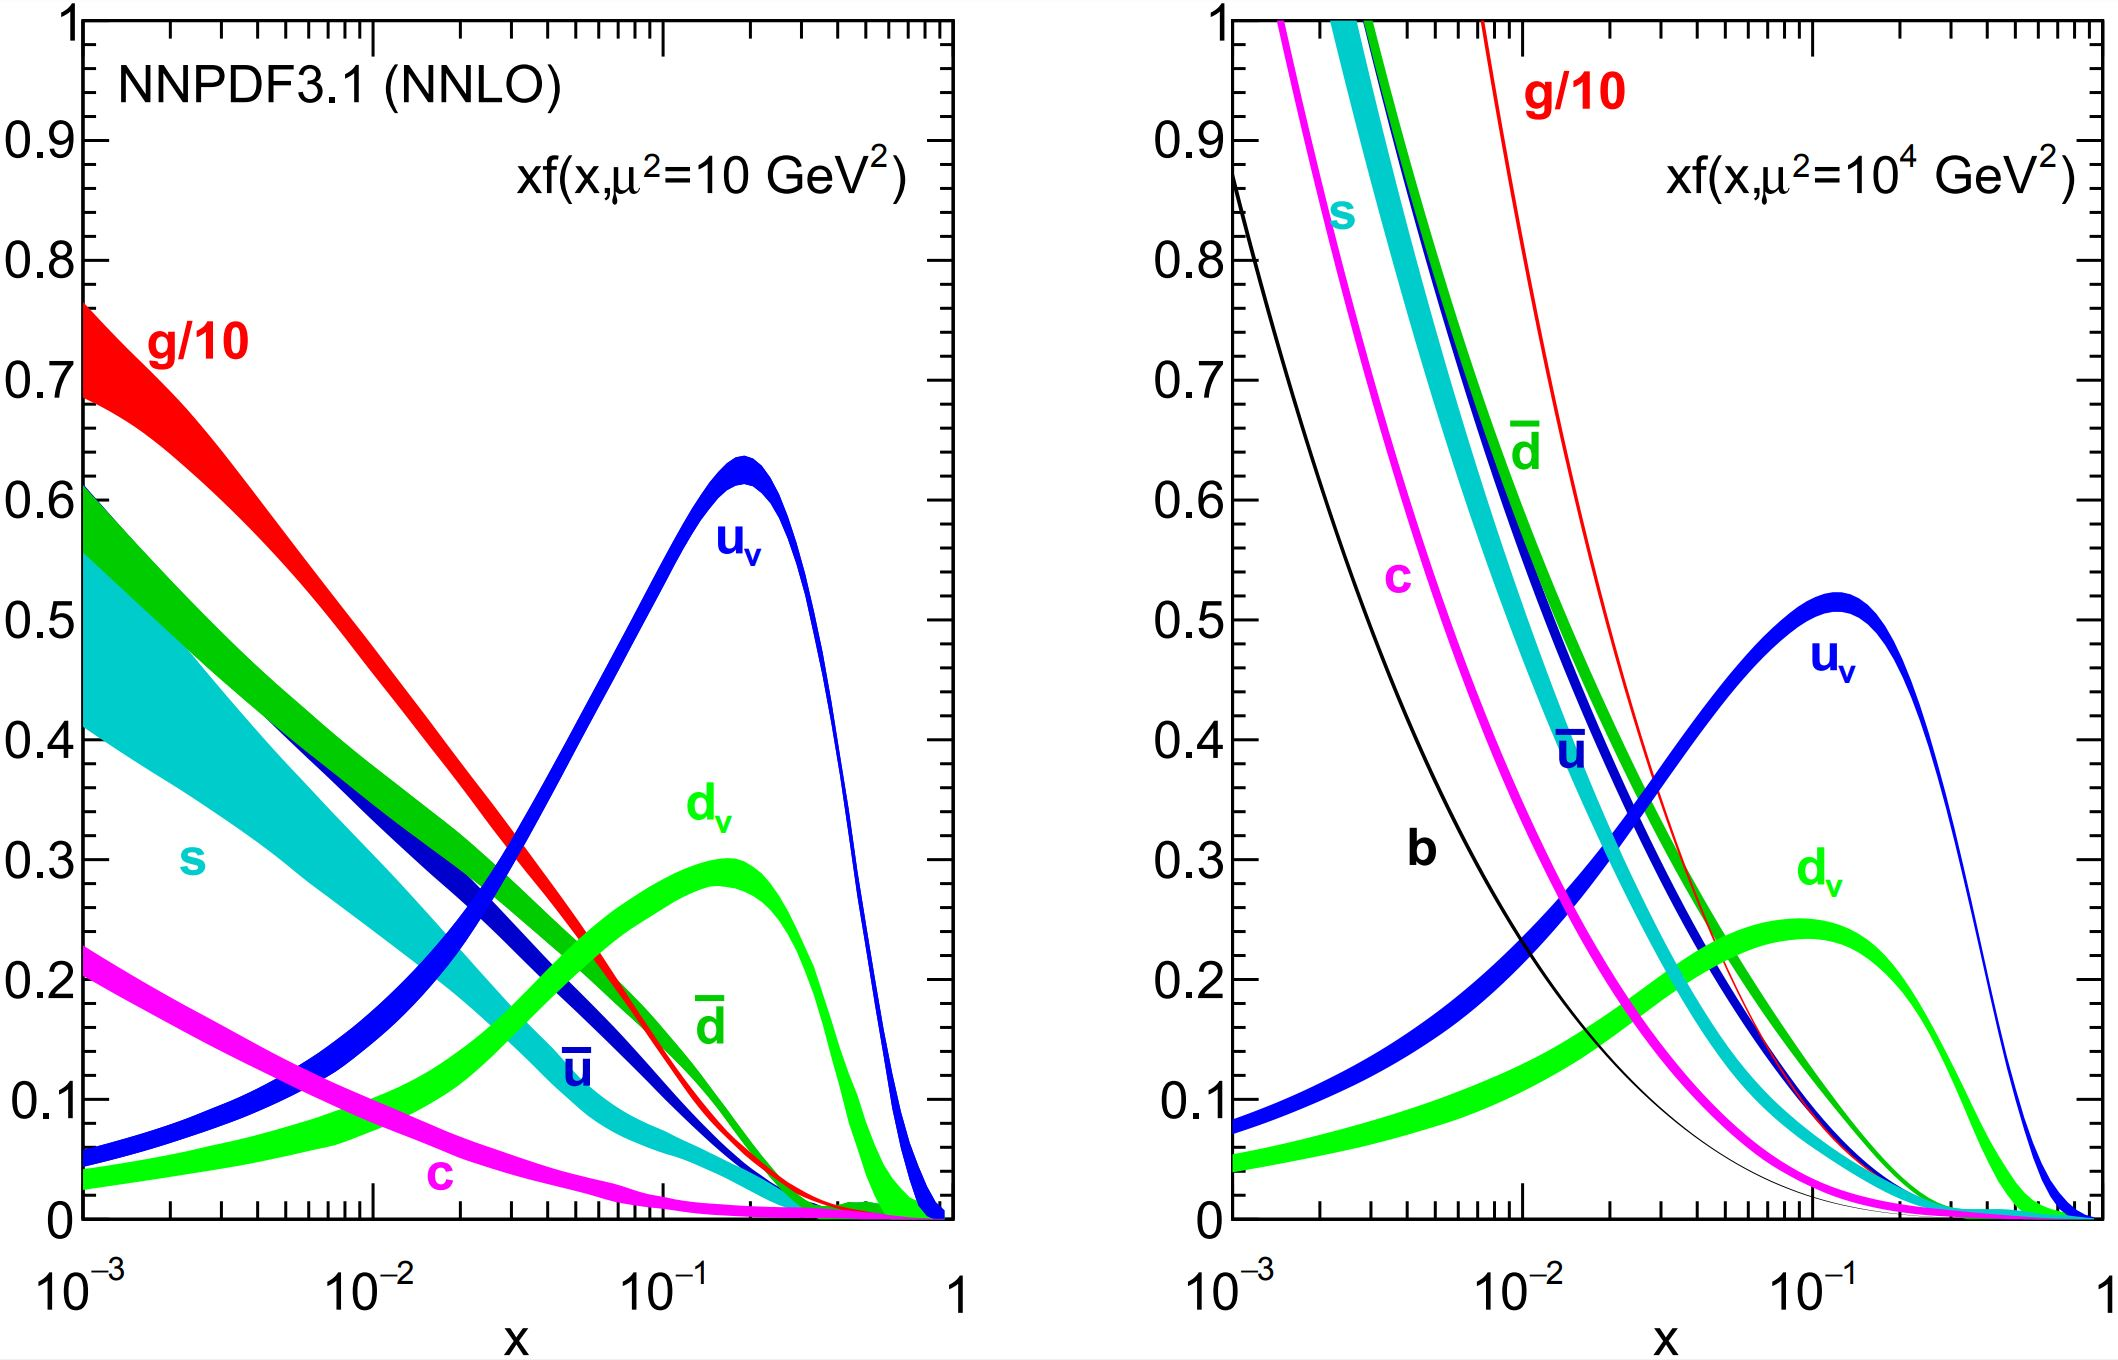
\includegraphics[width=1.0\textwidth]{EVENTSIM/NLOPDF.JPG}
    \caption{
        The parton distribution functions are shown for the factorisation scales $\mu_F^2=10$~GeV$^2$ (left) and $\mu_F^2=10$~TeV$^2$ (right) obtained with the \textit{NNPDF3.1NNLO} global analysis~\cite{Ball_2017}.}
    \label{figEVNTSIM:PDF}
    \end{center}
\end{figure}

\subsection{Matrix element}

The computation of the partonic cross-section of partons $i,j$ into an arbitrary final state $X$, is related to the \acrlong{MElabel}~(\acrshort{MElabel}) amplitude as

\begin{equation}
    \hat{\sigma}_{ij\to X} \sim \sum_{k=0}^{\infty} \int \text{d}\Phi_{X+k}\left|\sum_{l=0}^{\infty} M^l_{X+k}\right|^2(\Phi_F,\mu_F,\mu_R),
\end{equation}

where \acrshort{PDFlabel}s and other normalisation factors are removed for compactness. $M^l_{X+k}$ is the \acrshort{MElabel} amplitude for the production of $X$ in association with $k$ additional final-state partons, or legs, and with $l$ additional loop corrections. The quantity depends on the phase space $\Phi_F$ of the final state, as well as $\mu_F$ and $\mu_R$.\\

In a perturbative regime, the \acrshort{MElabel} amplitudes for increasingly complex processes (diagrams with additional legs and loops) tend to decrease. As a result, the cross-section is generally computed at a perturbative order, without the sum computed to infinity and for a choice of $\mu_F$ and $\mu_R$. The \acrlong{LOlabel}~(\acrshort{LOlabel}) is the lowest possible order for the calculation, with $k=l=0$. Next, $l=0,k=n$ provides the \acrshort{LOlabel} computation for the production of $X+n$ jets. Finally, $k+l\leq n$ corresponds to a N$^n$LO prediction for the production of $X$, while also to a N$^{n-k}$LO prediction for the production of $X+k$ jets.

\subsection{Parton shower}

One problem that arises in the fixed order computations of the differential cross-section is the appearance of logarithmic divergences from collinear splitting that originate from the integration of the phase space of the additional partons. For an inclusive cross-section computation, these divergences cancel out with virtual corrections order by order, following the KLN theorem~\cite{Masssingularities,PhysRev.133.B1549}.\\

In this case, the base event is simulated at fixed order while the \acrshort{QCD} emission process (splitting) is computed with the \acrshort{PSlabel} algorithm~\cite{FOX1980285}, 
which generates a sequence of emissions with decreasing angle or energy. The algorithm recursively produces the typical splitting processes ($g\to q\bar{q}$, $g\to gg$ and $q\to qg$) for each parton until the energy of the shower reaches $\sim$1~GeV, the hadronisation scale. This showering process that is applied to the final products after the hard-scattering is referred to as \acrlong{FSRlabel}~(\acrshort{FSRlabel}), while the simulation of the \acrlong{ISRlabel}~(\acrshort{ISRlabel}) is performed to the incoming partons. In the case of \acrshort{ISRlabel}, the subsequent emissions grow on energy and are modelled with a backwards-evolution algorithm~\cite{SJOSTRAND1985321}.\\

There is an incompatibility with \acrshort{MElabel} and \acrshort{PSlabel} for a full cross-section computation at order $n>1$, as there is a potential overlap in the phase space of the extra partons that are considered for the \acrshort{MElabel} at order $n$ with the ones considered in the splitting at order $n-1$. There are different approaches to solve the double counting, known as ME-PS matching. The most common strategy is known as slicing, which defines a matching scale where the higher energy region is covered only by the \acrshort{MElabel} while any additional parton with energy below that scale is vetoed and only covered with the \acrshort{PSlabel} algorithm. With this strategy, both energy regions are described with the corresponding optimal algorithm.

\subsection{Hadronisation}

The hadronisation process starts when the energy of the \acrshort{PSlabel} emissions is low enough to reach the hadronisation scale ($\sim$1~GeV), where the perturbative regime of \acrshort{QCD} is not valid. At that point, the partons from the \acrshort{PSlabel} have defined momentum, flavour and colour and further description of the emissions has to rely on phenomenological models. The process consists on a reconstruction algorithm that groups together the partons into different hadrons, that can further split, until all partons are confined into stable hadrons.\\

The two most widely used models are the Lund string model~\cite{ANDERSSON198331} and the cluster model~\cite{Winter2004}.
In the first, the quark-antiquark pair colour interaction is described as a string with a potential assumed to be linearly increasing with the distance, emulating the \acrshort{QCD} potential. The string then splits forming new quark-antiquark pairs when the energy stored passes the quark-antiquark total mass, forming hadrons whose momenta are determined from the initial momentum by a fragmentation function. On the other hand, the second model is based on forcing the final state gluons to split into quark-antiquark pairs and then grouping all quarks in colour-singlet clusters, allowed to decay and split into smaller clusters or hadrons. For both models, the process is repeated iteratively until only stable hadrons remain.

\subsection{Pile-up and underlying event}

Other interactions apart from the hard-scattering event have to be included in the \acrshort{MClabel} simulations to properly model the \acrshort{LHClabel} collisions, the pile-up and the underlying event. Both types of interactions mainly consist of soft \acrshort{QCD} interactions, the first arising from other protons colliding in the same or previous bunch-crossing while the second being the interaction of the other partons that do not originate the hard-scattering process. Both mainly consist of soft \acrshort{QCD} interactions in the forward region, close to the beam axis, and the simulation is based on the combination of phenomenological models and the configuration of the \acrshort{LHClabel} beam. In the special case of out-of-time pileup (interactions from previous bunch-crossings), the simulation has to take into account the time response of the detector.

\subsection{Monte Carlo simulation and generators}
\label{subsec:MCsimulation}
\acrlong{MClabel}~(\acrshort{MClabel}) generators are dedicated software tools to perform the \acrshort{MClabel} simulations, based on pseudorandom numbers to generate the events with the predicted distributions. They are generally classified according to the steps the simulation can perform, with general purpose generators being capable of simulating the whole event process, while dedicated generators target specific parts of the simulation chain, such as the \acrshort{MElabel} or the \acrshort{PSlabel} computation.\\

The full process involving \acrshort{MElabel} generation, \acrshort{PSlabel}, underlying event and hadronisation can be simulated by \acrshort{MClabel} generators like \PYTHIA~8~\cite{SJOSTRAND2015159}
, \HERWIG~7~\cite{Bahr2008,Bellm2016}
or \SHERPA~\cite{10.21468SciPostPhys.7.3.034}. However, \PYTHIA~8 provides leading order cross-section calculations which are often not sufficient and hence, the generator is typically used to compute the \acrshort{PSlabel} process, which is based on the Lund string model. On the other hand, \HERWIG~7 provides many \acrshort{MElabel} calculations at NLO, however since the fraction of negative event weights can be quite large (up to $\sim40\%$ for certain generator setups), the generator is also typically used for \acrshort{PSlabel} computation, based on the cluster model. \POWHEGBOX~\cite{Nason_2004,Frixione_2007,Alioli2010,PhysRevD.91.094003,Frixione_20072}
and \MGMCatNLO~\cite{Alwall_2007}
are examples of other generators that are especially designed to provide accurate high-order \acrshort{MElabel} calculations, which are typically interfaced with \PYTHIA~8 or \HERWIG~7 for the simulation of \acrshort{PSlabel} and hadronisation.\\

More in detail, these tools have parameters to describe the non-perturbative processes that can be tuned using collision data. The most common tunes used by the \acrshort{ATLASlabel} collaboration are the A14~\cite{ATL-PHYS-PUB-2014-021} parameters combined with \textit{NNPDF3.0LO} \acrshort{PDFlabel}s set~\cite{BALL2013244} for \PYTHIA~8 and the H7UE set~\cite{Bellm2016} with the \textit{MMHT2014LO} \acrshort{PDFlabel}s sets~\cite{Harland-Lang2015} for \HERWIG~7. Throughout this thesis different combinations of \acrshort{MClabel} generators and settings are used, and are detailed in the corresponding chapters. If not stated otherwise, the same parameters are shared. The mass of the top quark is set to $m_t=172.5$~GeV, the mass of the Higgs boson to $m_H=125$~GeV and the mass of the $b$-quark to $m_b=4.8$~GeV for \PYTHIA~8, to $m_b=4.5$~GeV for \HERWIG~7 and to $m_b=4.75$~GeV for \SHERPA. The simulation involving $b$- and $c$-hadron decays for \PYTHIA and \HERWIG is interfaced with \EVTGEN~\cite{LANGE2001152}. 

\section{Detector simulation}

With the proton-proton collisions simulated and the final-state stable particles defined, the remaining step is to simulate the interactions with the detector. The full \acrshort{ATLASlabel} detector simulation is performed in two steps: first, the \acrshort{ATLASlabel} detector response of the \acrshort{MClabel} output is simulated, and then the signals are reconstructed using the same algorithms used in real data. Figure~\ref{figEVNTSIM:detectorsim} depicts the different steps both for data and simulated \acrshort{MClabel} events.\\

\begin{figure}[htbp]
    \RawFloats
    \begin{center}
    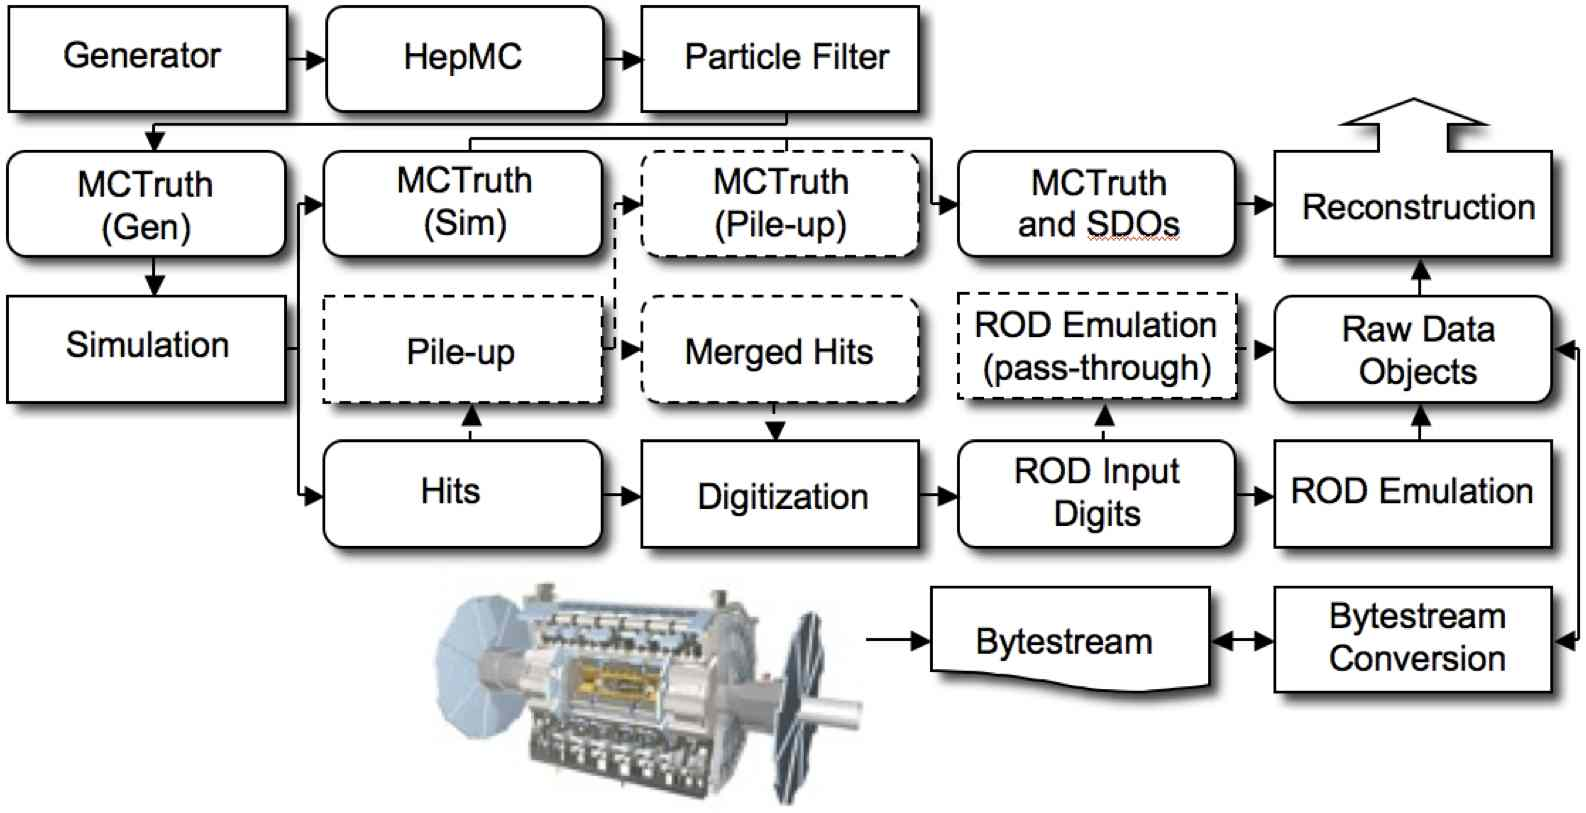
\includegraphics[width=1.0\textwidth]{EVENTSIM/detectorsim.png}
    \caption{
        Schematic of the different steps for the full reconstruction procedure of data and MC events. Data events start next to the ATLAS detector, while MC events start at the "Generator", both ending at the "Reconstruction" block~\cite{Aad_2010}.}
    \label{figEVNTSIM:detectorsim}
    \end{center}
\end{figure}

The \GEANT~4 package~\cite{AGOSTINELLI2003250} is widely used in physics to simulate the propagation and interaction of particles with matter. The simulation that includes all the geometry of the \acrshort{ATLASlabel} sub-detector systems with \GEANT~4 is referred to \textit{Full Simulation}~(FullSim), which is computationally expensive (several minutes per event) but gives the most accurate result. As more than 90\% of the dedicated CPU time is spent on the calorimeter simulations, fast alternatives are used in practice. The \textit{AtlFast-II} (AF-II) simulation is performed with faster simulation algorithms for the calorimeter simulation, \acrshort{ATLASlabel} Fast Calorimeter Simulation~(\textsc{FastCaloSim})~\cite{ATLAS:1300517}, and for the \acrshort{IDlabel} simulation, Fast \acrshort{ATLASlabel} Tracking Simulation~(\textsc{Fatras})~\cite{Edmonds:1091969}. The rest of the systems is simulated with \GEANT~4 adding significantly less CPU time than the calorimeter or ID simulation while maintaining an adequate level of accuracy.\\

Finally, the normalisation of a \acrshort{SMlabel} process is normally chosen according to the cross-section at the highest-order calculation available and other corrections are applied in the form of scale factors (SFs), derived from the ratio between data and \acrshort{MClabel} in specific calibration regions.